\documentclass[
a4paper,
oneside,
10pt,
fleqn,
headsepline,
toc=listofnumbered, 
bibliography=totocnumbered]{scrartcl}

% deutsche Trennmuster etc.
\usepackage[T1]{fontenc}
\usepackage[utf8]{inputenc}
\usepackage[english, ngerman]{babel} % \selectlanguage{english} if  needed
\usepackage{lmodern} % use modern latin fonts

% Custom commands
\newcommand{\GITHUB}{https://github.com/jklaiber/HSR}
\newcommand{\LICENSEURL}{https://en.wikipedia.org/wiki/Beerware}
\newcommand{\LICENSE}{
"THE BEER-WARE LICENSE" (Revision 42):
Julian Klaiber and Severin Dellsperger wrote this file. As long as you retain this notice you
can do whatever you want with this stuff. If we meet some day, and you think
this stuff is worth it, you can buy us a beer in return.
}

% Jede Überschrift 1 auf neuer Seite
\let\stdsection\section
\renewcommand\section{\clearpage\stdsection}

% Multiple Authors
\usepackage{authblk}

% Include external pdf
\usepackage{pdfpages}

% Layout / Seitenränder
\usepackage{geometry}

% Inhaltsverzeichnis
\usepackage{makeidx} 
\makeindex

\usepackage{url}
\usepackage[pdfborder={0 0 0}]{hyperref}
\usepackage[all]{hypcap}
\usepackage{hyperxmp} % for license metadata

% Glossar und Abkürzungsverzeichnis
\usepackage[acronym,toc,nopostdot]{glossaries}
\setglossarystyle{altlist}
\usepackage{xparse}
\DeclareDocumentCommand{\newdualentry}{ O{} O{} m m m m } {
	\newglossaryentry{gls-#3}{
		name={#4 : #5},
		text={#5\glsadd{#3}},
		description={#6},
		#1
	}
	\makeglossaries
	\newacronym[see={[Siehe:]{gls-#3}},#2]{#3}{#4}{#5\glsadd{gls-#3}}
}
\makeglossaries

% Mathematik
\usepackage{amsmath}
\usepackage{amssymb}
\usepackage{amsfonts}
\usepackage{enumitem}

% Images
\usepackage{graphicx}
\graphicspath{{images/}} % default paths

% Boxes
\usepackage{fancybox}

%Tables
\usepackage{tabu}
\usepackage{booktabs} % toprule, midrule, bottomrule
\usepackage{array} % for matrix tables
\usepackage{multicol} %multicol

% Header and footer
\usepackage{scrlayer-scrpage}
\setkomafont{pagehead}{\normalfont}
\setkomafont{pagefoot}{\normalfont}
\automark*{section}
\clearpairofpagestyles
\ihead{\headmark}
\ohead{\AUTHOR}
\cfoot{\pagemark}

% Pseudocode
\usepackage{algorithmic}
\usepackage[linesnumbered,ruled]{algorithm2e}

% Code Listings
\usepackage{listings}
\usepackage{color}
\usepackage{beramono}

\definecolor{bluekeywords}{rgb}{0,0,1}
\definecolor{greencomments}{rgb}{0,0.5,0}
\definecolor{redstrings}{rgb}{0.64,0.08,0.08}
\definecolor{xmlcomments}{rgb}{0.5,0.5,0.5}
\definecolor{types}{rgb}{0.17,0.57,0.68}

\lstdefinestyle{visual-studio-style}{
	language=[Sharp]C,
	columns=flexible,
	showstringspaces=false,
	basicstyle=\footnotesize\ttfamily, 
	commentstyle=\color{greencomments},
	morekeywords={partial, var, value, get, set},
	keywordstyle=\bfseries\color{bluekeywords},
	stringstyle=\color{redstrings},
	breaklines=true,
	breakatwhitespace=true,
	tabsize=4,
	numbers=left,
	numberstyle=\tiny\color{black},
	frame=lines,
	showspaces=false,
	showtabs=false,
	escapeinside={£}{£},
}

\definecolor{DarkPurple}{rgb}{0.4, 0.1, 0.4}
\definecolor{DarkCyan}{rgb}{0.0, 0.5, 0.4}
\definecolor{LightLime}{rgb}{0.3, 0.5, 0.4}
\definecolor{Blue}{rgb}{0.0, 0.0, 1.0}

\lstdefinestyle{cevelop-style}{
	language=C++,  
	columns=flexible,
	showstringspaces=false,     
	basicstyle=\footnotesize\ttfamily, 
	keywordstyle=\bfseries\color{DarkPurple},
	commentstyle=\color{LightLime},
	stringstyle=\color{Blue}, 
	escapeinside={£}{£}, % latex scope within code      
	breaklines=true,
	breakatwhitespace=true,
	showspaces=false,
	showtabs=false,
	tabsize=4,
	morekeywords={include,ifndef,define},
	numbers=left,
	numberstyle=\tiny\color{black},
	frame=lines,
}

\lstdefinestyle{eclipse-style}{
	language=Java,  
	columns=flexible,
	showstringspaces=false,     
	basicstyle=\footnotesize\ttfamily, 
	keywordstyle=\bfseries\color{DarkPurple},
	commentstyle=\color{LightLime},
	stringstyle=\color{Blue}, 
	escapeinside={£}{£}, % latex scope within code      
	breaklines=true,
	breakatwhitespace=true,
	showspaces=false,
	showtabs=false,
	tabsize=4,
	morekeywords={length},
	numbers=left,
	numberstyle=\tiny\color{black},
	frame=lines,
}
\lstset{style=eclipse-style}



% Theorems \begin{mytheo}{title}{label}
\usepackage{tcolorbox}
\tcbuselibrary{theorems}
\newtcbtheorem[number within=section]{definiton}{Definition}%
{fonttitle=\bfseries}{def}
\newtcbtheorem[number within=section]{remember}{Merke}%
{fonttitle=\bfseries}{rem}
\newtcbtheorem[number within=section]{hint}{Hinweis}%
{fonttitle=\bfseries}{hnt}

% Colors
\definecolor{strings}{HTML}{448c25}
\definecolor{comments}{HTML}{aaaaaa}
\definecolor{keywords}{HTML}{aa3d8c}
\definecolor{background}{HTML}{f4f4f4}
\definecolor{numbers}{HTML}{a884e0}

% Default style
\lstdefinestyle{default}{
    backgroundcolor=\color{background},
    basicstyle=\ttfamily\small,
    breakatwhitespace=true,
    breaklines=true,
    commentstyle=\color{comments},
    deletekeywords={},
    escapeinside={}{},
    extendedchars=true,
    frame=lines,
    keepspaces=true,
    keywordstyle=\color{keywords},
    morekeywords={},
    numbers=left,
    numberstyle=\ttfamily\color{numbers},
    rulecolor=\color{numbers},
    showspaces=false,
    showstringspaces=false,
    showtabs=false,
    stepnumber=1,
    stringstyle=\color{strings},
    tabsize=2,
}
\lstset{
    style=default,
    columns=fullflexible
}

% Language cisco-config
\lstdefinelanguage{cisco-config}{
    morekeywords={no,ip,ipv6,int,interface},
    morecomment=[l][\color{comments}]{!},
    numbers=none
}

% Language cisco-teminal
\lstdefinelanguage{cisco-terminal}{
    morecomment=[l][\color{strings}]{\#},
    morecomment=[l][\color{strings}]{>},
    numbers=none
}

\lstdefinelanguage{bash}{
    numbers=none
}

\makeatletter
\@addtoreset{section}{part}
\makeatother

% Boxes
\tcbuselibrary{most}

\usepackage{fontawesome}

% \cmd{...}
\newcommand{\cmd}[1]{\texttt{#1}}

% Info Box
\definecolor{infobar}{HTML}{02cefc}
\definecolor{infobackground}{HTML}{baf0fc}
\newcommand{\info}[2]{
    \begin{tcolorbox}[
        arc = 0mm,
        boxrule = 0pt,
        breakable,
        before skip=11pt,
        before skip=11pt,
        title = \faInfo~#1,
        fonttitle = \sffamily\bfseries,
        coltitle = white,
        colbacktitle = infobar,
        colback = infobackground,
        toptitle=2mm,
        bottomtitle=2mm,
        top=4mm,
        bottom=4mm
    ]
    #2
    \end{tcolorbox}
}

% Warning Box
\definecolor{warnbar}{HTML}{f90053}
\definecolor{warnbackground}{HTML}{fcc4d7}
\newcommand{\warn}[2]{
    \begin{tcolorbox}[
        arc = 0mm,
        boxrule = 0pt,
        breakable,
        before skip=11pt,
        before skip=11pt,
        title = \faWarning~#1,
        fonttitle = \sffamily\bfseries,
        coltitle = white,
        colbacktitle = warnbar,
        colback = warnbackground,
        toptitle=2mm,
        bottomtitle=2mm,
        top=4mm,
        bottom=4mm
    ]
    #2
    \end{tcolorbox}
}

% Login Information Box
\definecolor{loginbar}{HTML}{FA8A05}
\definecolor{loginbackground}{HTML}{F3D4AF}
\newcommand{\login}[2]{
    \begin{tcolorbox}[
        arc = 0mm,
        boxrule = 0pt,
        breakable,
        before skip=11pt,
        before skip=11pt,
        title = \faKey~#1,
        fonttitle = \sffamily\bfseries,
        coltitle = white,
        colbacktitle = loginbar,
        colback = loginbackground,
        toptitle=2mm,
        bottomtitle=2mm,
        top=4mm,
        bottom=4mm
    ]
    #2
    \end{tcolorbox}
}

\definecolor{settingborder}{HTML}{0066CC}
\definecolor{settingcontent}{HTML}{E5F2FA}
\newcommand{\setting}[1]{
    \begin{tcolorbox}[
        colback = settingcontent,
        colframe = settingborder
    ]
    You can find the settings under: \\
    \textbf{\clicks{~#1}}
    \end{tcolorbox}
}

\definecolor{configurationborder}{HTML}{005700}
\definecolor{configurationcontent}{HTML}{e6ffcc}
\newcommand{\configuration}[2]{
    \begin{tcolorbox}[
        colback = configurationcontent,
        colframe = configurationborder
    ]
    \textbf{Configuration:}\\
    To reach an output like below you only have to add/change the following parameters 
    ~#1
    You can find the settings under: \\
    \textbf{\clicks{~#2}}
    \end{tcolorbox}
}


\usepackage{multirow}

% URLs
\urlstyle{rm}
\definecolor{link}{HTML}{0450f2}
\hypersetup{
    colorlinks,
    allcolors=.,
    urlcolor=link,
}

% \url[display]{url} or \url{url}
\renewcommand{\url}[2][]{%
    \ifstrempty{#1}{%
        \burlalt{#2}{#2}%
    }{%
        \burlalt{#1}{#2}%
    }%
}

% Clicks
\newcommand{\clicks}[1]{%
    $\foreach \n [count=\ni] in {#1}{%
        \ifnum\ni=1%
            \textit{\n}%
        \else%
            \rightarrow \textit{\n}%
        \fi%
    }$%
}

% Keystrokes
\newcommand{\keys}[1]{%
    $\foreach \n [count=\ni] in {#1}{%
        \ifnum\ni=1%
            \textit{\n}%
        \else%
            + \textit{\n}%
        \fi%
    }$%
}

% Dokumentinformationen
\newcommand{\SUBJECT}{Codebeispiele}
\newcommand{\TITLE}{C++}

% pdf metadata
\hypersetup{
	pdfauthor={\AUTHOR},
	pdftitle={\SUBJECT \TITLE},
	pdfcopyright={\LICENSE},
	pdflicenseurl={\LICENSEURL}
}

\begin{document}
	
\begin{titlepage}

\newcommand{\HRule}{\rule{\linewidth}{0.5mm}} % Defines a new command for the horizontal lines, change thickness here

\center % Center everything on the page
 
%----------------------------------------------------------------------------------------
%	HEADING SECTIONS
%----------------------------------------------------------------------------------------

\textsc{\LARGE \INSTITUTE}\\[1.5cm] % Name of your university/college
\textsc{\Large \SUBJECT}\\[0.5cm] % Major heading such as course name

%----------------------------------------------------------------------------------------
%	TITLE SECTION
%----------------------------------------------------------------------------------------

\HRule \\[0.6cm]
{ \huge \bfseries \TITLE}\\[0.4cm] % Title of your document
\HRule \\[1.5cm]

%----------------------------------------------------------------------------------------
%	AUTHOR SECTION
%----------------------------------------------------------------------------------------

\begin{minipage}{0.4\textwidth}
\begin{flushleft} \large
\emph{Author:}\\
\AUTHORONE % Your name
\end{flushleft}
\end{minipage}
~
\begin{minipage}{0.4\textwidth}
\begin{flushright} \large
\emph{} \\
\AUTHORTWO
\end{flushright}
\end{minipage}\\[2cm]

%----------------------------------------------------------------------------------------
%	DATE SECTION
%----------------------------------------------------------------------------------------

{\large \today}\\[2cm] % Date, change the \today to a set date if you want to be precise

%----------------------------------------------------------------------------------------
%	LOGO SECTION
%----------------------------------------------------------------------------------------


\includegraphics[width=10cm,height=5cm,keepaspectratio]{ressources/hsr_logo.jpg}\\[1cm] 
 
%----------------------------------------------------------------------------------------

\vfill % Fill the rest of the page with whitespace

\end{titlepage} 	


\lstset{style=cevelop-style}

\begin{document}
\section{Drill questions}
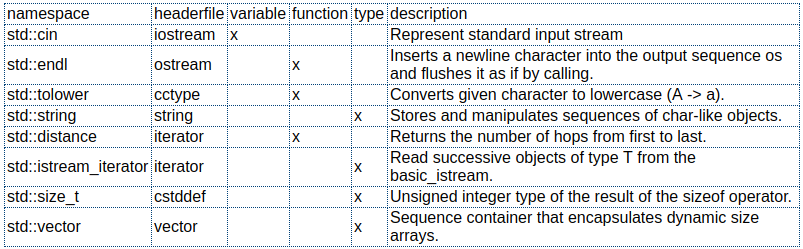
\includegraphics[keepaspectratio,width=\textwidth,height=\textheigh t]{images/1}
\subsection{Element Iteration}
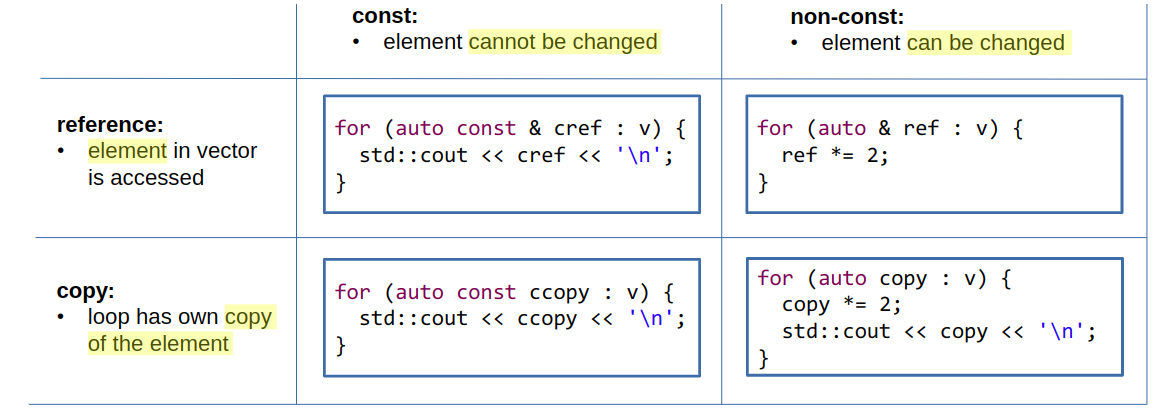
\includegraphics[keepaspectratio,width=\textwidth,height=\textheigh t]{images/2}
\section{Stack and Queue}
\begin{lstlisting}[language=C++]
#include <stack> 
#include <queue> 
#include <iostream> 
#include <string> 

int main() { 
	std::stack<std::string> lifo{}; 
	std::queue<std::string> fifo{}; 
	for (std::string s : { "Fall", "leaves", "after", "leaves", "fall" }) { 
		lifo.push(s); 
		fifo.push(s); 
	} 
	while (!lifo.empty()) { // fall leaves after leaves Fall 
		std::cout << lifo.top() << ' '; 
		lifo.pop(); } std::cout << '\n'; 
		while (!fifo.empty()) {// Fall leaves after leaves fall 
			std::cout << fifo.front() << ' '; 
			fifo.pop(); 
		} 
	} 
}
\end{lstlisting}
\section{MAP}
\subsection{counting word}
\begin{lstlisting}[language=C++]
#include <map>
#include <iostream> 
#include <string> 

int main(){ 
	std::map<std::string, size_t> words{}; 
	std::string s{}; 
	
	while (std::cin >> s) { 
	++words[s]; 
	} 
	for(auto const & p : words) { 
	std::cout << p.first << " = "<< p.second << '\n'; 
	} 
}
\end{lstlisting}
\section{Istream and Ostream}
\subsection{robust reading of an int value}
\begin{lstlisting}[language=C++]
int inputAge(std::istream & in) { 
	while (in.good()) { 
		std::string line{}; 
		getline(in, line); 
		std::istringstream is{line}; 
		int age{-1}; 
		if (is >> age) { 
		return age; 
		} 
	} 
	return -1; 
}
\end{lstlisting}
\subsection{Implementing Read}
\begin{lstlisting}[language=C++]
class Date { 
	int year, month, day; 
public: 
	std::istream & read(std::istream & is) { 
			int year{-1}, month{-1}, day{-1}; 
			char sep1, sep2; 
			//read values 
			is >> year >> sep1 >> month >> sep2 >> day; 
		try { 
			Date input{year, month, day}; 
			//overwrite content of this object (copy-ctor) 
			(*this) = input; 
			//clear stream if read was ok 
			is.clear(); 
		} catch (std::out_of_range const & e) { 
			//set failbit 
			is.setstate(std::ios::failbit); 
		} 
		return is; 
	} 
}; 
\end{lstlisting}
\subsection{Implementing Print}
Date.h
\begin{lstlisting}[language=C++]
#include <ostream> 

class Date { 
	int year, month, day; 
public: 
	std::ostream & print(std::ostream & os) const {
	os << year << "/" << month << "/" << day;
	return os; 
   }
}; 
inline std::ostream & operator<<(std::ostream & os, Date const & date) {
	return date.print(os);
}  
\end{lstlisting}
Any.cpp
\begin{lstlisting}[language=C++]
#include "Date.h" 
#include <iostream> 

void foo() { 
	std::cout << Date::myBirthday; 
} 
\end{lstlisting}


\section{Count}
\subsection{non-whitespace Chars}
char.h
\begin{lstlisting}[language=C++]
#include <iosfwd>
int charcount(std::istream &in);
\end{lstlisting}
char.cpp
\begin{lstlisting}[language=C++]
int charcount(std::istream &in){
    std::string line{};
    std::getline(input, line);
    line.erase(remove(line.begin(), line.end(),' '),line.end()); 
    return line.size();
}
\end{lstlisting}
main.cpp
\begin{lstlisting}[language=C++]
#include <charc.h>
#include <iostream>
int main(){
    std::cout << charc(std::cin) << '\n';
}
\end{lstlisting}
without loop char.cpp
\begin{lstlisting}[language=C++]
int charcount(std::istream &in){
  using initer = std::istream_iterator<char>;
  return std::vector<char>{initer{in},initer{}}.size();
}
\end{lstlisting}
\subsection{all Chars}
header
\begin{lstlisting}[language=C++]
int allcharcount(std::istream &in){
}
\end{lstlisting}
cpp
\begin{lstlisting}[language=C++]
void allcharc(std::istream & in, std::ostream & out) {
	char c { };
	int counter { 0 };
	while (in.get() >> c && in.eof() == false) {
		counter++;
	}
	out << counter;
}
\end{lstlisting}
without loop cpp
\begin{lstlisting}[language=C++]
int allcharcount(std::istream &in){
}
void allcharc(std::istream & in, std::ostream & out) {
	std::noskipws (in);
	std::istream_iterator<char> input {in};
	std::istream_iterator<char> eos{};
	out << std::distance(input, eos);
}
\end{lstlisting}
\subsection{Words}
header
\begin{lstlisting}[language=C++]
int wordcount(std::istream &in){
}
\end{lstlisting}
cpp
\begin{lstlisting}[language=C++]
void wc(std::istream & in, std::ostream & out) {
	std::string word{};
	int counter{0};
	while (in >> word) {
		counter++;
	}
	out << counter;
}
\end{lstlisting}
\subsection{Lines}
header
\begin{lstlisting}[language=C++]
int linecount(std::istream &in){
}
\end{lstlisting}
cpp
\begin{lstlisting}[language=C++]
void lc(std::istream & in, std::ostream & out) {
	std::string line{};
	int counter{0};
	while (!in.eof()) {
	std::getline(in, line);
	counter++;
	}
	out << counter;
}
\end{lstlisting}
\section{Testat 1}
\subsection{calc.cpp}
\begin{lstlisting}[language=C++]
#include "calc.h"
#include <exception>
#include <istream>
int calc(int lhs, int rhs, char op) {
	switch(op) {
	    case '+' : return lhs + rhs;
	    case '-' : return lhs - rhs;
	    case '*' : return lhs * rhs;
	    case '/' :
	    case '%':
			if(rhs == 0)
			{
				throw std::invalid_argument{"Modulo by zero"};
			}
			else
			{
				if(op ==  '/')
				{
					return lhs / rhs;
				}
				else
				{
					return lhs % rhs;
				}
			}
	    default: throw std::invalid_argument{"Invalid Argument"};
	}
}
int calc(std::istream& in)
{
	int lhs{}, rhs{};
	char op{};
	if(in >> lhs >> op >> rhs)
	{
		return calc(lhs, rhs, op);
	}

	throw std::invalid_argument{"Invalid Argument!"};
}
\end{lstlisting}
\subsection{calc.h}
\begin{lstlisting}[language=C++]
#ifndef CALC_H_
#define CALC_H_
#include <iosfwd>

int calc(int lhs, int rhs, char op);
int calc(std::istream& in);

#endif /* CALC_H_ */
\end{lstlisting}
\subsection{pocketcalculator.cpp}
\begin{lstlisting}[language=C++]
#include "pocketcalculator.h"
#include "calc.h"
#include "sevensegment.h"
#include <iostream>
#include <exception>
#include <string>
#include <sstream>

const unsigned MAXDIGITLENGTH{8};

void startCalculator(std::ostream &out, std::istream &in)
{
	std::string line{};
	while(getline(in, line))
	{
	 std::istringstream argument{line};
		try {
			int result = calc(argument);
			std::string digits = std::to_string(result);
			if(digits.length() <= MAXDIGITLENGTH)
			{
				printLargeNumber(result, out);
			}
			else
			{
				throw std::length_error{"Too many digits"};
			}
		} catch (...) {
			printErrorMessage(out);
		}
	}
}
\end{lstlisting}
\subsection{pocketcalculator.h}
\begin{lstlisting}[language=C++]
#ifndef POCKETCALCULATOR_H_
#define POCKETCALCULATOR_H_
#include <iosfwd>

void startCalculator(std::ostream &out, std::istream &in);

#endif /* POCKETCALCULATOR_H_ */
\end{lstlisting}
\subsection{sevensegment.cpp}
\begin{lstlisting}[language=C++]
#include "sevensegment.h"
#include <ostream>
#include <algorithm>
#include <vector>
#include <string>
void printLargeNumber(int i, std::ostream &out)
{	std::string number = std::to_string(i);
	if(i > 0)
	{
			for(int line = 0; line < 5; line++)
			{

				std::for_each(number.begin(), number.end(), [&out, line](auto digit){
					digit = digit - '0';
					out << digitsvector.at(digit).at(line);
				});
				out << '\n';
			}
	}
	else
	{
		for(int line = 0; line < 5; line++)
				{

					std::for_each(number.begin(), number.end(), [&out, line](auto symbol){
						if(symbol == '-' )
							{
								out << minusvector.at(line);
							}
						else
							{
								symbol = symbol - '0';
								out << digitsvector.at(symbol).at(line);
							}

					});
					out << '\n';
				}
	}

}
void printErrorMessage(std::ostream &out)
{
	std::for_each(errorvector.begin(), errorvector.end(), [&out](auto line)
			{
				out << line << '\n';
			});
}
void printLargeDigit(int i, std::ostream &out)
{
	std::vector<std::string> number = digitsvector.at(i);

				std::for_each(std::begin(number), std::end(number), [&out](auto line) {
					out << line << '\n';
				});
}
\end{lstlisting}
\subsection{sevensegment.h}
\begin{lstlisting}[language=C++]
#ifndef SEVENSEGMENT_H_
#define SEVENSEGMENT_H_
#include <iosfwd>
#include <vector>
#include <string>

	const std::vector<std::vector<std::string>> digitsvector{
		std::vector<std::string>{" - ", "| |", "   ", "| |", " - "},
		std::vector<std::string>{"   ", " | ", "   ", " | ", "   "},
		std::vector<std::string>{" - ", "  |", " - ", "|  ", " - "},
		std::vector<std::string>{" - ", "  |", " - ", "  |", " - "},
		std::vector<std::string>{"   ", "| |", " - ", "  |", "   "},
		std::vector<std::string>{" - ", "|  ", " - ", "  |", " - "},
		std::vector<std::string>{" - ", "|  ", " - ", "| |", " - "},
		std::vector<std::string>{" - ", "  |", "   ", "  |", "   "},
		std::vector<std::string>{" - ", "| |", " - ", "| |", " - "},
		std::vector<std::string>{" - ", "| |", " - ", "  |", " - "}
	};

	const std::vector<std::string> errorvector
	{

		{" -             "},
		{"|              "},
		{" -  -  -  -  - "},
		{"|  |  |  | ||  "},
		{" -        -    "}
	};

	const std::vector<std::string> minusvector
		{
		{" "},
		{" "},
		{"-"},
		{" "},
		{" "}
		};

void printLargeDigit(int i, std::ostream &out);
void  printLargeNumber(int i, std::ostream &out);
void printErrorMessage(std::ostream &out);

#endif /* SEVENSEGMENT_H_ */
\end{lstlisting}
\section{Testat 2}
\subsection{word.h}
\begin{lstlisting}[language=C++]
#ifndef WORD_H_
#define WORD_H_

#include <algorithm>
#include <iosfwd>
#include <string>
#include <cctype>
#include <vector>

namespace word {
	class Word {
		std::string word {};
	public:
		Word() noexcept = default;
		explicit Word(std::string const &s);
		std::istream & read(std::istream & is);
		std::ostream & print(std::ostream & os) const;
		bool operator==(Word const & rhs) const;
		bool operator<(Word const & rhs) const;
	private:
		bool static isValidWord(std::string s);
	};

	std::istream & operator>>(std::istream & is, Word & word);
	std::ostream & operator<<(std::ostream & os, Word const & word);
	std::ostream & operator<<(std::ostream & os, std::vector<Word> const & l);

	inline bool operator>(Word const & lhs, Word const & rhs) {
		return rhs < lhs;
	}
	inline bool operator>=(Word const & lhs, Word const & rhs) {
		return !(lhs < rhs);
	}
	inline bool operator<=(Word const & lhs, Word const & rhs) {
		return !(rhs < lhs);
	}
	inline bool operator!=(Word const & lhs, Word const & rhs) {
		return !(rhs == lhs);
	}
}

#endif /* WORD_H_ */
\end{lstlisting}
\subsection{word.cpp}
\begin{lstlisting}[language=C++]
#include "word.h"

#include <algorithm>

#include <cctype>
#include <iosfwd>
#include <stdexcept>
#include <string>
#include <iterator>

namespace word {
Word::Word(std::string const &s) {
	if (s.empty()) {
		throw std::invalid_argument("Word cannot be initialized with an empty string!");
	}
	if (!isValidWord(s)) {
		throw std::invalid_argument("Word must contain only alphanumeric chars!");
	}
	word = s;
}

bool Word::isValidWord(std::string s) {
	return std::all_of(s.begin(), s.end(), [](char c) {return std::isalpha(c);});
}

std::istream & Word::read(std::istream & is) {
	while (!isalpha(is.peek()) && !is.eof()) {
		is.ignore();
	}
	std::string temp { };
	while (isalpha(is.peek()) && !is.eof()) {
		temp += is.get();
	}
	if (!temp.empty()) {
		if (isValidWord(temp)) {
			word.clear();
			word = temp;
			is.clear();
		} else {
			is.setstate(std::ios::failbit);
		}
	}
	return is;
}
bool Word::operator==(Word const & rhs) const {

	return std::equal(word.begin(), word.end(), rhs.word.begin(), rhs.word.end(), [](auto left, auto right)
			{
				return tolower(left) == tolower(right);
			});
}
bool Word::operator<(Word const & rhs) const {
	return std::lexicographical_compare(word.begin(), word.end(), rhs.word.begin(), rhs.word.end(), [](char a, char b) {
		return tolower(a) < tolower(b);
	});
}

std::ostream & Word::print(std::ostream & os) const {
	os << word;
	return os;
}

std::istream & operator>>(std::istream & is, Word & word) {
	return word.read(is);
}

std::ostream & operator<<(std::ostream & os, Word const & word) {
	return word.print(os);
}
}
\end{lstlisting}
\subsection{kwic.cpp}
\begin{lstlisting}[language=C++]
#include "kwic.h"
#include "word.h"
#include <iosfwd>
#include <iterator>
#include <ostream>
#include <sstream>
#include <string>
#include <vector>
#include <algorithm>

using namespace word;

namespace word {
std::ostream & operator<<(std::ostream & os, std::vector<Word> const & l) {
	std::copy(std::begin(l), std::end(l), std::ostream_iterator<Word>{os, " "});
	return os;
}
}

namespace kwic {
	std::vector<std::vector<Word>> rotate(std::vector<std::vector<Word>> const & input) {
		std::vector<std::vector<Word>> rotated {};
		std::for_each(begin(input), end(input), [&](std::vector<Word> toRotate) {
			for (auto it = begin(toRotate); it != end(toRotate); it++) {
				std::vector<Word> rotatedLine { toRotate.size() };
				std::rotate_copy(
					std::begin(toRotate), it, std::end(toRotate),
					std::begin(rotatedLine));
				rotated.push_back(rotatedLine);
			}
		});
		std::sort(rotated.begin(), rotated.end());
		return rotated;
	}
	void kwic(std::istream & in, std::ostream & out) {
		std::vector<std::vector<Word>> lines {};
		std::string inputLine {};
		while(std::getline(in, inputLine)) {
			std::istringstream lineStream { inputLine };
			std::istream_iterator<Word> wordIterator { lineStream }, eof {};
			lines.push_back(std::vector<Word> { wordIterator, eof });
		}
		std::vector<std::vector<Word>> rotatedLines = rotate(lines);

		std::copy(
			std::begin(rotatedLines),
			std::end(rotatedLines),
			std::ostream_iterator<std::vector<Word>>(out, "\n"));

//		std::for_each(begin(rotatedLines), end(rotatedLines), [&out](std::vector<Word> line) {
//			//out << line << '\n';
//		});
	}
}
\end{lstlisting}
\subsection{kwic.h}
\begin{lstlisting}[language=C++]
#ifndef KWIC_H_
#define KWIC_H_
#include <iosfwd>

namespace kwic {
	void kwic(std::istream & in, std::ostream & out);
}

#endif /* KWIC_H_ */
\end{lstlisting}
\section{Testat 3}
\subsection{indexableSet.h}
\begin{lstlisting}[language=C++]
#ifndef SRC_INDEXABLESET_H_
#define SRC_INDEXABLESET_H_

#include <functional>
#include <set>
#include <iterator>
#include <stdexcept>

template<typename T, typename COMPARE = std::less<T>>
struct indexableSet: std::set<T, COMPARE> {
	using container = std::set<T,COMPARE>;
	using container::container;
	using const_reference = typename container::const_reference;

public:
	const_reference at(int index) const {
		if (index < 0) {
			index += this->size();
		}
		if (static_cast<unsigned>(index) >= this->size()) {
			throw std::out_of_range { "index out of range!" };
		}

		return *std::next(this->begin(), index);
	}

	const_reference operator[](int index) const {
		return at(index);
	}

	const_reference front() const {
		return at(0);
	}

	const_reference back() const {
		return at(-1);
	}
};
#endif /* SRC_INDEXABLESET_H_ */
\end{lstlisting}
\subsection{Test.cpp}
\begin{lstlisting}[language=C++]
#include "cute.h"
#include "ide_listener.h"
#include "xml_listener.h"
#include "cute_runner.h"
#include "indexableSet.h"

#include <functional>
#include <iterator>
#include <string>
#include <vector>
#include <algorithm>
#include <cctype>

void emptyContainerTest() {
	indexableSet<int, std::less<int>> empty { };
	ASSERT_EQUAL(0, empty.size());
}

void resultingSizeTest() {
	std::vector<std::string> input { "Banana", "Apple", "Strawberry", "Ananas" };
	indexableSet<std::string> const fruits { std::begin(input), std::end(input) };
	ASSERT_EQUAL(4, fruits.size());
}

void ascendingOrderRangeConstructorTest() {
	indexableSet<std::string> fruits { "Banana", "Apple", "Strawberry", "Ananas" };
	std::vector<std::string> expected { "Ananas", "Apple", "Banana", "Strawberry" };
	std::vector<std::string> actual { std::begin(fruits), std::end(fruits) };
	ASSERT_EQUAL(expected, actual);
}

void descendingOrderRangeConstructorTest() {
	indexableSet<std::string> fruits { "Banana", "Apple", "Strawberry", "Ananas" };
	std::vector<std::string> expected { "Strawberry", "Banana", "Apple", "Ananas" };
	std::vector<std::string> actual { std::rbegin(fruits), std::rend(fruits) };
	ASSERT_EQUAL(expected, actual);
}

void copyConstructorTest() {
	indexableSet<std::string> const fruits { "Banana", "Apple", "Strawberry", "Ananas" };
	indexableSet<std::string> const copy { fruits };
	ASSERT_EQUAL(4, copy.size());
}

void atTooLargeIndex() {
	indexableSet<std::string> const fruits { "Banana", "Apple", "Strawberry", "Ananas" };
	ASSERT_THROWS(fruits.at(4), std::out_of_range);
}

void atTooSmallIndex() {
	indexableSet<std::string> const fruits { "Banana", "Apple", "Strawberry", "Ananas" };
	ASSERT_THROWS(fruits.at(-8), std::out_of_range);
}

void initializerConstructorTest() {
	indexableSet<std::string> const fruits { "Banana", "Apple", "Strawberry", "Ananas" };
	ASSERT_EQUAL(4, fruits.size());
}

void atPositiveIndicesTest() {
	indexableSet<std::string> const fruits { "Banana", "Apple", "Strawberry", "Ananas" };
	ASSERT_EQUAL("Strawberry", fruits.at(3));
}

void atNegativeIndicesTest() {
	indexableSet<std::string> const fruits { "Banana", "Apple", "Strawberry", "Ananas" };
	ASSERT_EQUAL("Banana", fruits.at(-2));
}

void frontEmptyExceptionTest() {
	indexableSet<std::string> const empty { };
	ASSERT_THROWS(empty.front(), std::out_of_range);
}

void frontNotEmptyTest() {
	indexableSet<std::string> const fruits { "Banana", "Apple", "Strawberry", "Ananas" };
	ASSERT_EQUAL("Ananas", fruits.front());
}

void backEmptyExceptionTest() {
	indexableSet<std::string> const empty { };
	ASSERT_THROWS(empty.back(), std::out_of_range);
}

void backNotEmptyTest() {
	indexableSet<std::string> const fruits { "Banana", "Apple", "Strawberry", "Ananas" };
	ASSERT_EQUAL("Strawberry", fruits.back());
}

void iteratorOrderTest() {
	indexableSet<std::string, std::greater<>> fruits { "Banana", "Apple", "Strawberry", "Ananas" };
	std::vector<std::string> expected { "Strawberry", "Banana", "Apple", "Ananas" };
	ASSERT_EQUAL_RANGES(std::begin(expected), std::end(expected), std::begin(fruits), std::end(fruits));
}

void returningByIndexAndValueTest() {
	indexableSet<int> const values { 15 };
	ASSERT_EQUAL(&values.at(0), &values[0]);
}

void FrontBackReferenceTest() {
	indexableSet<int> const values { 15 };
	ASSERT_EQUAL(&values.front(), &values.back());
}

struct caselessCompare {
	bool operator()(std::string const &left, std::string const &right) const {
		return std::lexicographical_compare(left.begin(), left.end(), right.begin(), right.end(), [](char c1, char c2)
		{
			return std::tolower(c1) < std::tolower(c2);
		});
	}
};

void caselessComparatorTest1() {
	indexableSet<std::string, caselessCompare> set { "a", "B", "c" };
	ASSERT_EQUAL("a", set[0]);
}

void caselessComparatorTest2() {
	indexableSet<std::string, caselessCompare> set { "A", "B", "c" };
	ASSERT_EQUAL("B", set[1]);
}

void caselessComparatorTest3() {
	indexableSet<std::string, caselessCompare> set { "A", "B", "c" };
	ASSERT_EQUAL("c", set[2]);
}

void caselessComparatorTest4() {
	indexableSet<std::string, caselessCompare> set {"A", "a"};
	ASSERT_EQUAL(1, set.size());
}

bool runAllTests(int argc, char const *argv[]) {
	cute::suite s { };
	//TODO add your test here
	s.push_back(CUTE(emptyContainerTest));
	s.push_back(CUTE(copyConstructorTest));
	s.push_back(CUTE(resultingSizeTest));
	s.push_back(CUTE(ascendingOrderRangeConstructorTest));
	s.push_back(CUTE(atTooLargeIndex));
	s.push_back(CUTE(atTooSmallIndex));
	s.push_back(CUTE(initializerConstructorTest));
	s.push_back(CUTE(descendingOrderRangeConstructorTest));
	s.push_back(CUTE(frontNotEmptyTest));
	s.push_back(CUTE(frontEmptyExceptionTest));
	s.push_back(CUTE(backEmptyExceptionTest));
	s.push_back(CUTE(backNotEmptyTest));
	s.push_back(CUTE(atPositiveIndicesTest));
	s.push_back(CUTE(atNegativeIndicesTest));
	s.push_back(CUTE(iteratorOrderTest));
	s.push_back(CUTE(returningByIndexAndValueTest));
	s.push_back(CUTE(FrontBackReferenceTest));
	s.push_back(CUTE(caselessComparatorTest1));
	s.push_back(CUTE(caselessComparatorTest2));
	s.push_back(CUTE(caselessComparatorTest3));
	s.push_back(CUTE(caselessComparatorTest4));

	cute::xml_file_opener xmlfile(argc, argv);
	cute::xml_listener<cute::ide_listener<>> lis(xmlfile.out);
	auto runner = cute::makeRunner(lis, argc, argv);
	bool success = runner(s, "AllTests");
	return success;
}

int main(int argc, char const *argv[]) {
	return runAllTests(argc, argv) ? EXIT_SUCCESS : EXIT_FAILURE;
}

\end{lstlisting}
\end{document}